
\documentclass[11pt,a4paper]{article}
\usepackage[margin=2.2cm]{geometry}
\usepackage[utf8]{inputenc}
\usepackage[T1]{fontenc}
\usepackage{amsmath,amssymb,mathtools,bm}
\usepackage{graphicx,booktabs,longtable,array,microtype,xcolor,hyperref,fancyhdr,enumitem}
\graphicspath{{../images/}}
\definecolor{navy}{HTML}{17324D}\definecolor{rust}{HTML}{A33A2B}\definecolor{green}{HTML}{176B4D}
\hypersetup{colorlinks=true,linkcolor=navy,urlcolor=rust,citecolor=green}
\pagestyle{fancy}\fancyhf{}\lhead{Auditoria estrutural da RH}\rhead{Dossiê técnico}\cfoot{\thepage}
\newcommand{\Drad}{\mathfrak D_{\mathrm{rad}}}
\newcommand{\Dpar}{\Delta_{\mathrm{par}}}
\newcommand{\status}[2]{\par\noindent\colorbox{#1!12}{\textcolor{#1}{\textbf{#2}}}\quad}
\begin{document}

\begin{titlepage}\centering
{\sffamily\bfseries\Huge Auditoria do ponto de ruptura\par}\vspace{.5cm}
{\Large Detector geométrico, defeito radial, forma de Weil e teste de circularidade\par}
\vfill
{\large Dossiê matemático e programa de pesquisa\par}\vspace{.3cm}
{\small Documento deliberadamente não reivindica uma prova da Hipótese de Riemann.\par}
\vfill{\large Agosto de 2026}\end{titlepage}
\tableofcontents\clearpage

\section{Escopo e regra de auditoria}
Este dossiê organiza o material fornecido em quatro classes: \textbf{provado}, \textbf{certificado finito}, \textbf{equivalente à RH} e \textbf{conjectural}. O objetivo é tornar explícita a passagem que ainda falta, sem converter evidência numérica ou uma definição algébrica em prova global.

\section{Geometria local do par funcional}
Escreva
\[\rho=\tfrac12+\delta+i\gamma,\qquad \rho^\sharp=1-\overline\rho=\tfrac12-\delta+i\gamma.\]
Defina
\[R_c^2=\gamma^2+\tfrac14,\quad R_+^2=R_c^2+\delta+\delta^2,\quad R_-^2=R_c^2-\delta+\delta^2.\]
Então
\[\delta=\frac{R_+^2-R_-^2}{2},\qquad \Dpar=\frac{R_+^2+R_-^2}{2}-R_c^2=\delta^2.\]
\begin{figure}[ht]\centering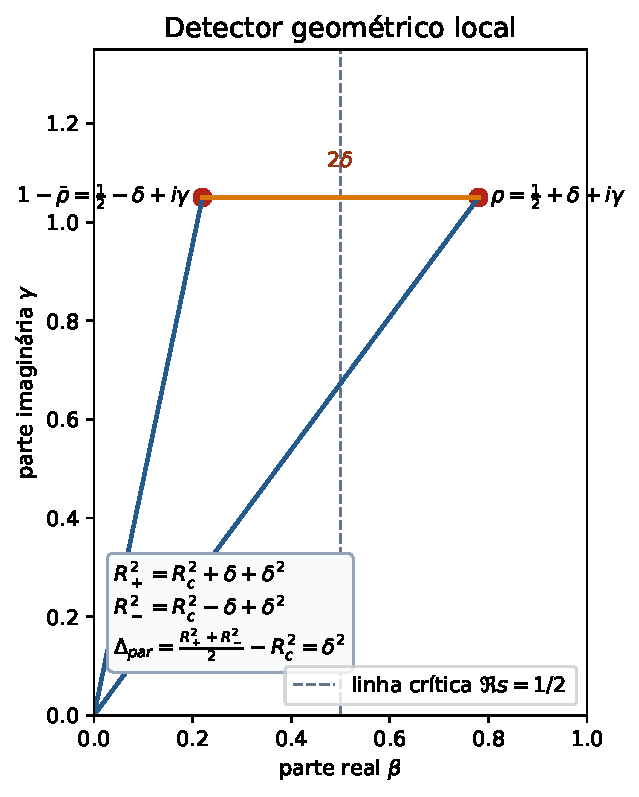
\includegraphics[width=.85\linewidth]{01-detector-geometrico.pdf}\caption{Detector geométrico local.}\end{figure}

\section{Simetrias e quartetos}
Fora da linha crítica, as simetrias por conjugação e pela equação funcional geram, em geral, um quarteto. Cada elemento possui o mesmo valor do peso radial definido adiante.
\begin{figure}[ht]\centering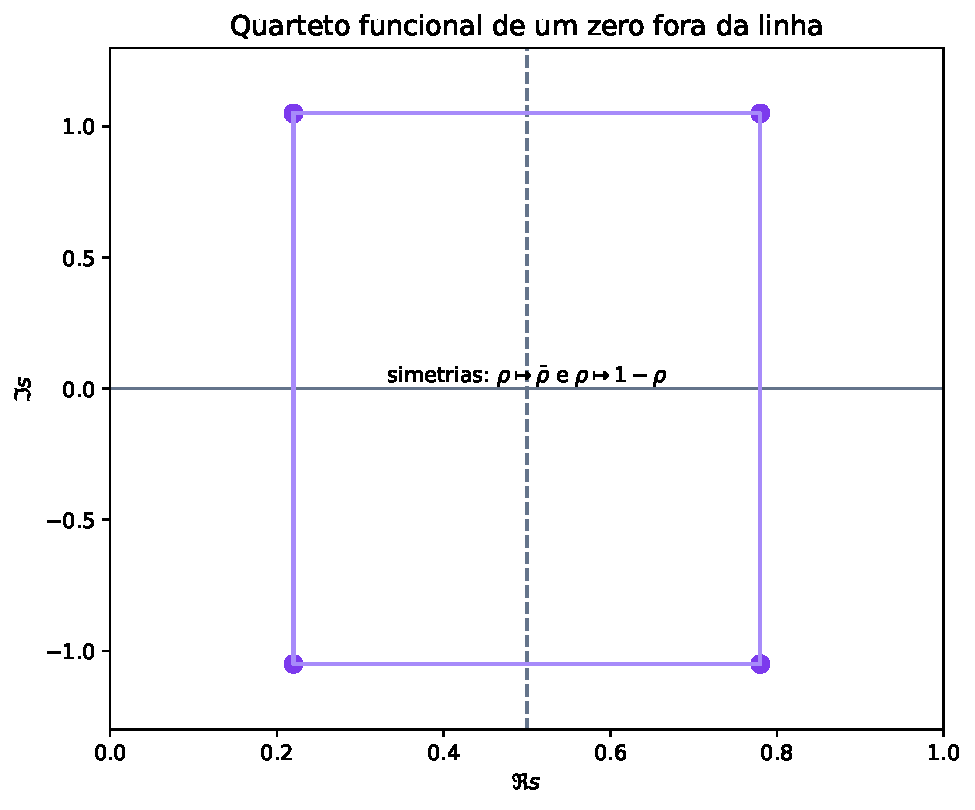
\includegraphics[width=.72\linewidth]{02-quarteto-simetrias.pdf}\caption{Quarteto associado a um desvio transversal.}\end{figure}

\section{Denominador e peso radial}
Com $A=\gamma^2+\tfrac14+\delta^2$,
\[P(\delta,\gamma)=|\rho|^2|1-\rho|^2=A^2-\delta^2,\qquad
w(\delta,\gamma)=\frac{2\delta^2}{P(\delta,\gamma)}.\]
Logo $w\ge0$ e, no domínio não trivial, $w=0$ se e somente se $\delta=0$. Para um quarteto completo, $W_4=4w$.
\begin{figure}[ht]\centering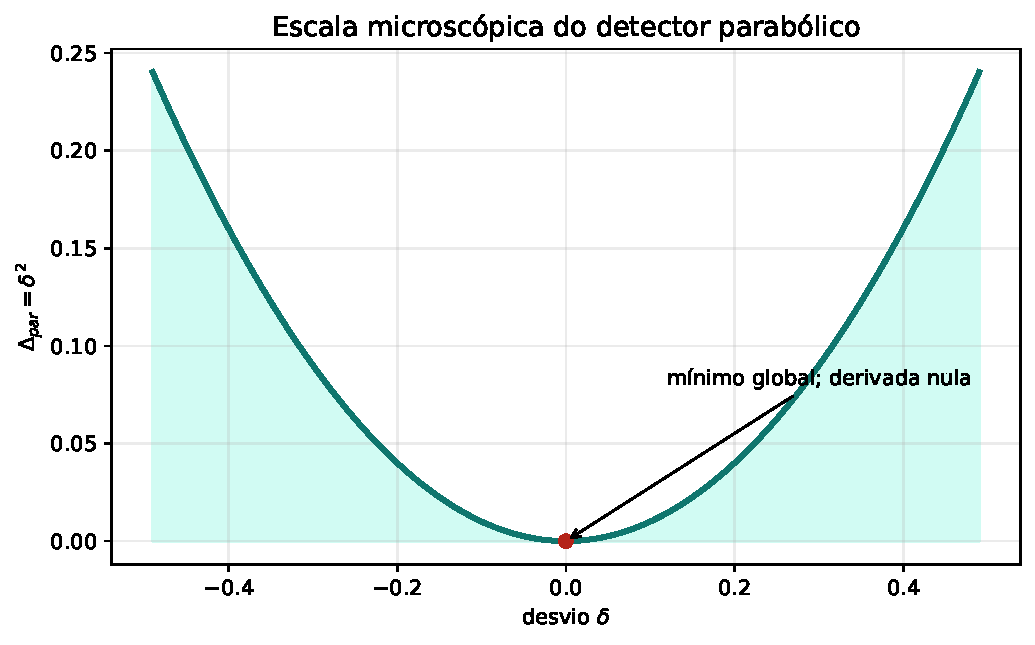
\includegraphics[width=.82\linewidth]{03-parabola-delta.pdf}\caption{O detector é exatamente quadrático.}\end{figure}
\begin{figure}[ht]\centering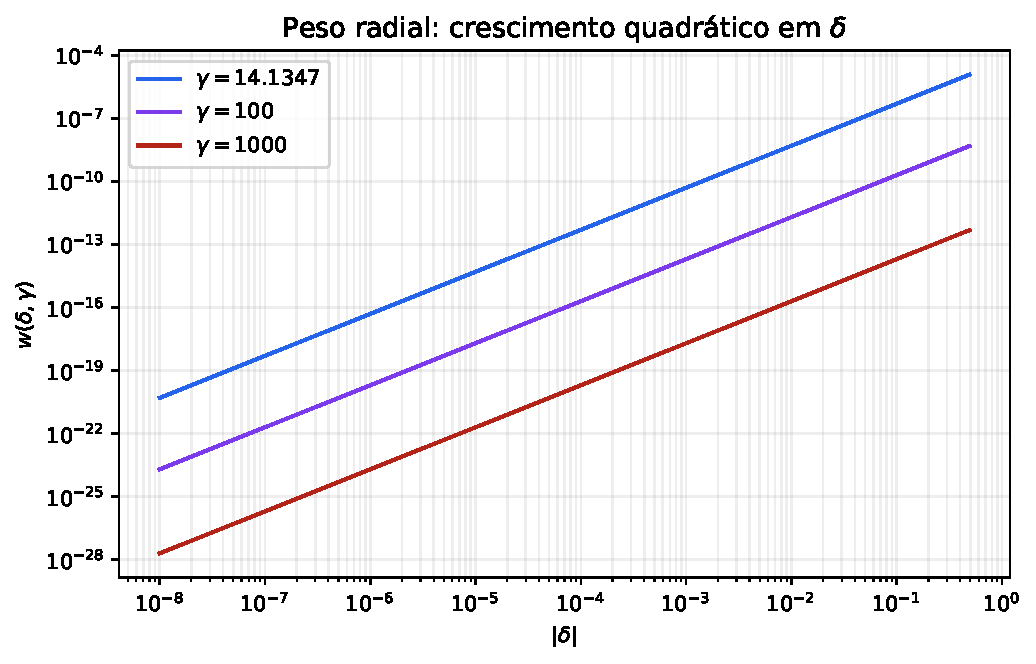
\includegraphics[width=.82\linewidth]{04-peso-versus-delta.pdf}\caption{Dependência do peso em $\delta$.}\end{figure}

\section{Regime de grande altura}
Para $\gamma\to\infty$ e $\delta$ fixo,
\[w(\delta,\gamma)=\frac{2\delta^2}{\gamma^4}-\frac{4\delta^2(\tfrac14+\delta^2)}{\gamma^6}+O(\gamma^{-8}).\]
O decaimento $\gamma^{-4}$ explica por que um zero muito alto, mesmo fora da linha, pode produzir perturbação extremamente pequena num detector radial truncado.
\begin{figure}[ht]\centering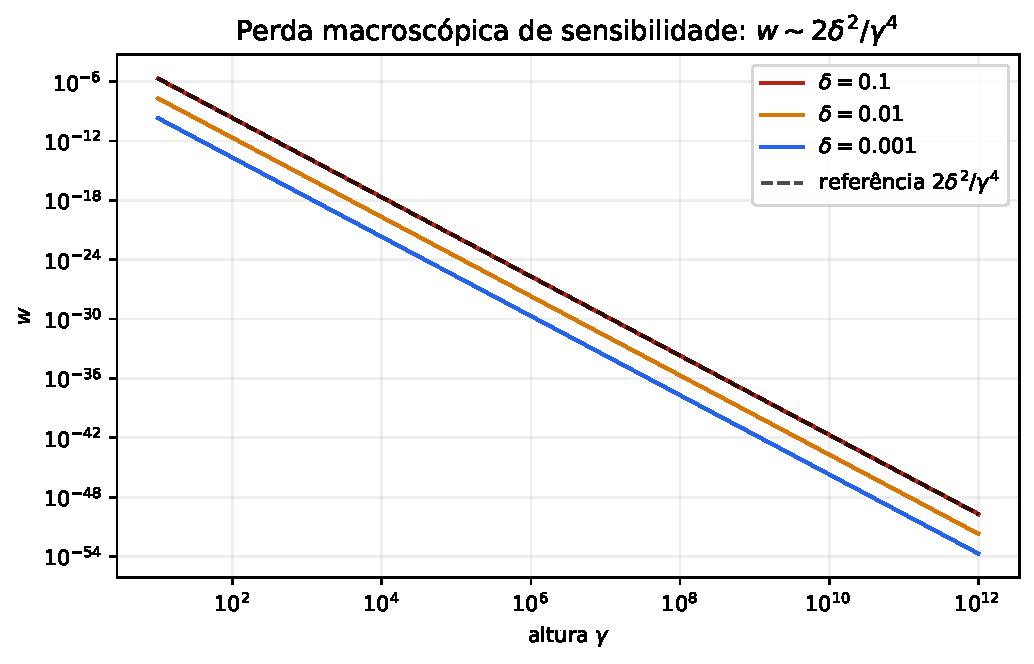
\includegraphics[width=.82\linewidth]{05-decaimento-gamma.pdf}\caption{Decaimento macroscópico.}\end{figure}
\begin{figure}[ht]\centering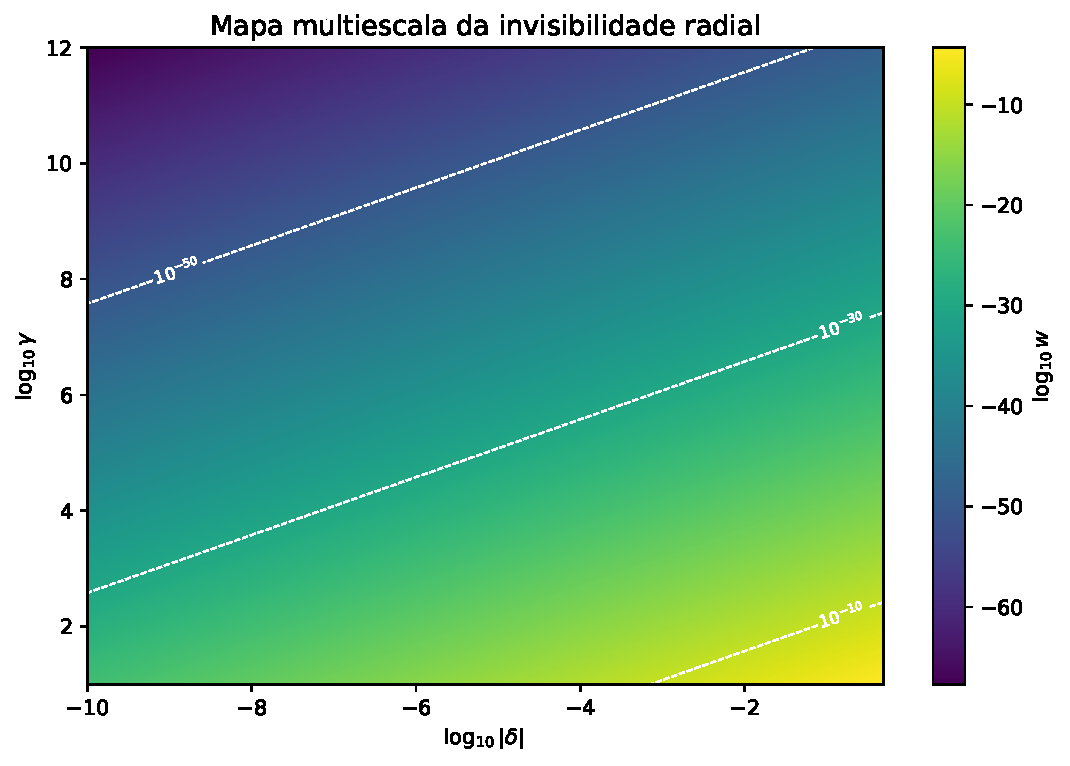
\includegraphics[width=.88\linewidth]{06-mapa-log-peso.pdf}\caption{Mapa multiescala de $w$.}\end{figure}

\section{Condicionamento numérico}
A identidade por raios é exata, mas o cálculo de $\delta^2$ por subtração de grandezas de ordem $\gamma^2$ é mal condicionado. Uma estimativa representativa é
\[\kappa_{\mathrm{pair}}\approx\frac{2\gamma^2}{\delta^2}.\]
Portanto, cálculos confiáveis devem usar $\delta=\beta-\tfrac12$ diretamente ou aritmética intervalar de precisão arbitrária.
\begin{figure}[ht]\centering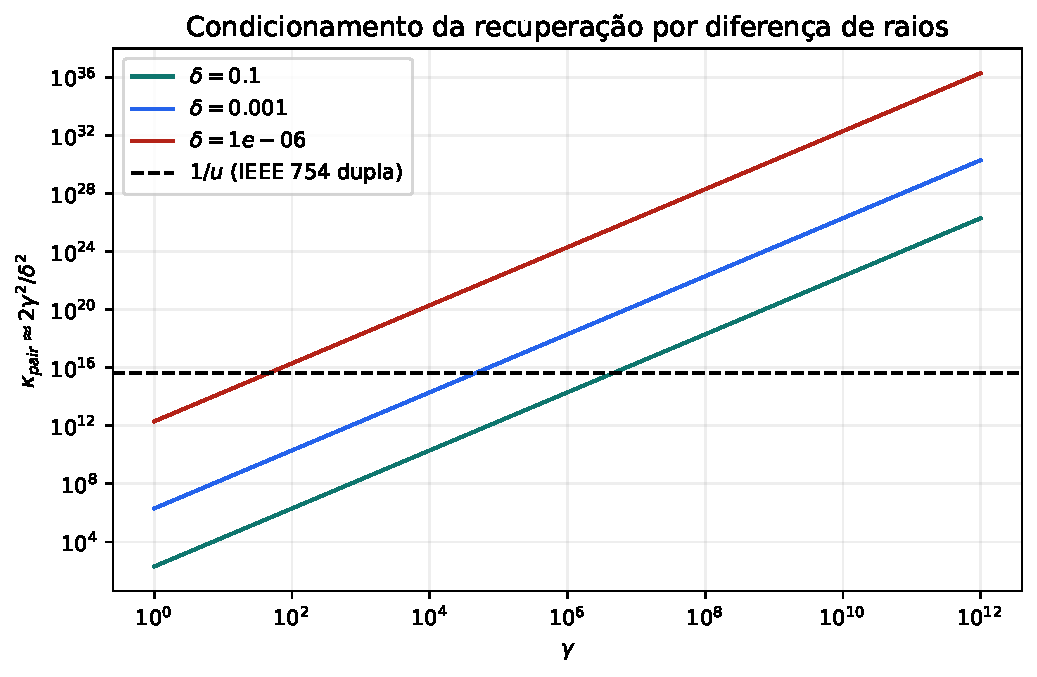
\includegraphics[width=.84\linewidth]{07-condicionamento.pdf}\caption{Explosão do número de condição.}\end{figure}

\section{Identidade radial e ruptura não holomorfa}
Considere a constante
\[C_\xi=2+\gamma_E-\log(4\pi).\]
A fórmula de Hadamard e a equação funcional controlam somas holomorfas do tipo $\sum_\rho[\rho(1-\rho)]^{-1}$. A quantidade $\sum_\rho|\rho|^{-2}$ mistura $\rho$ e $\overline\rho$ e, por isso, não é obtida automaticamente pelas fórmulas explícitas holomorfas usuais. A diferença positiva é codificada por
\[\Drad=\sum_\rho \frac{2(\Re\rho-\tfrac12)^2}{|\rho|^2|1-\rho|^2}=\sum_\rho w(\rho).\]
Sob convergência e contagem de multiplicidades adequadas, $\Drad=0$ equivale a todos os termos serem nulos, portanto à RH.
\begin{figure}[ht]\centering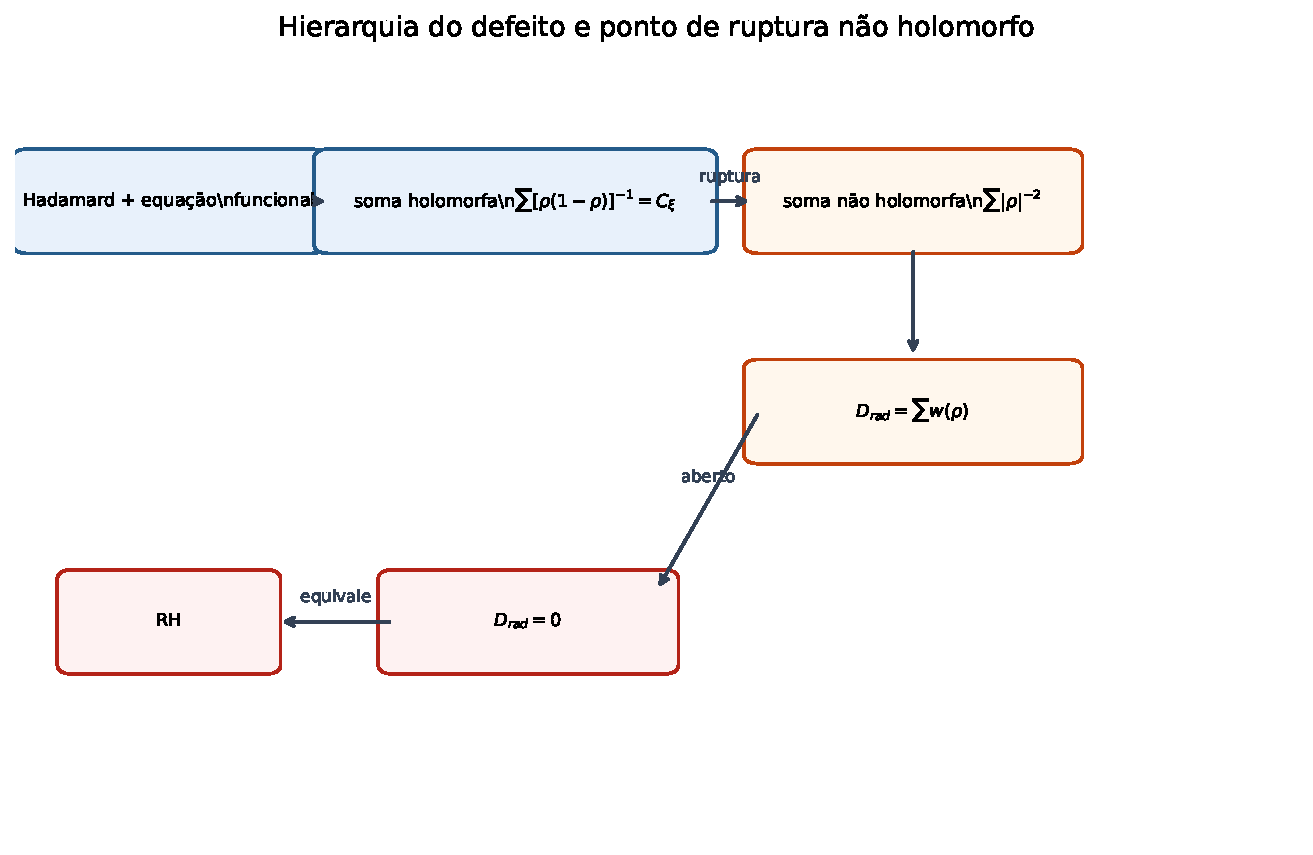
\includegraphics[width=.94\linewidth]{08-hierarquia-defeito.pdf}\caption{A ruptura é a passagem ao termo não holomorfo.}\end{figure}

\section{Critério de Weil e matrizes truncadas}
Para funções teste admissíveis, o critério de Weil afirma que a positividade global da forma $Q_W$ é equivalente à RH. Uma família finita $\{\phi_j\}_{j=1}^N$ produz uma matriz de Gram hermitiana
\[(G_N)_{ij}=Q_W(\phi_i,\phi_j).\]
Certificar $G_N\succeq0$ para valores isolados de $N$ é evidência finita; para concluir positividade global ainda são necessários densidade da união dos espaços, continuidade de $Q_W$ e controle uniforme dos erros.
\begin{figure}[ht]\centering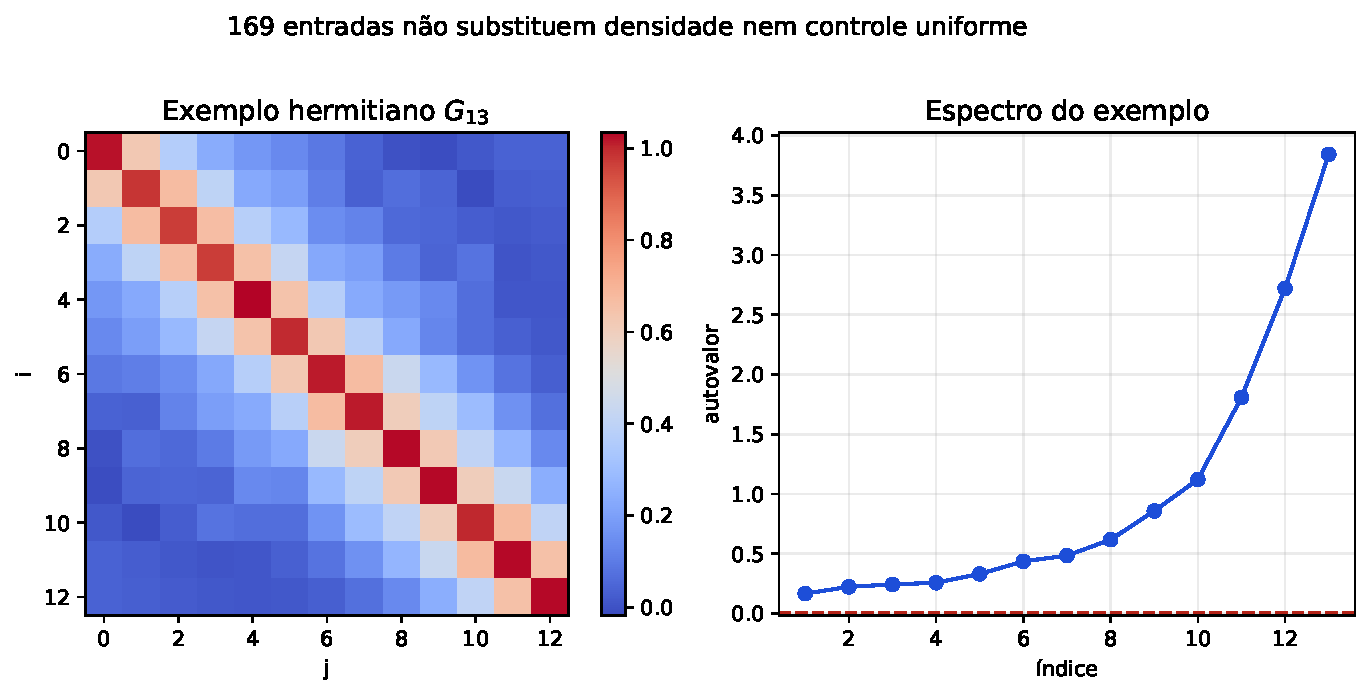
\includegraphics[width=.95\linewidth]{12-matriz-g13.pdf}\caption{Exemplo ilustrativo de uma matriz hermitiana $13\times13$; não representa dados certificados.}\end{figure}

\section{As três vias de fechamento}
\begin{figure}[ht]\centering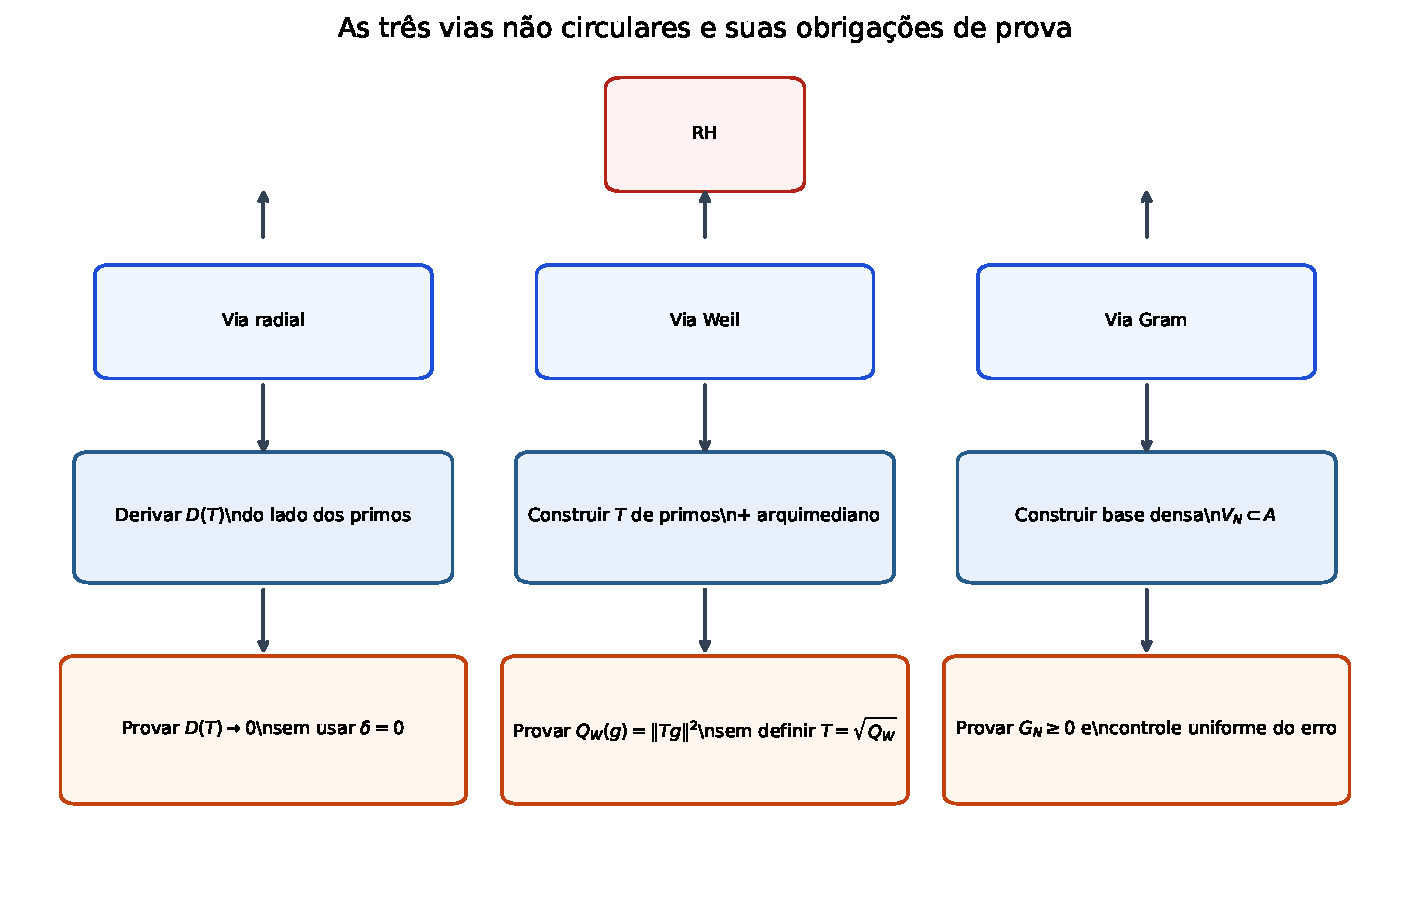
\includegraphics[width=.98\linewidth]{10-tres-vias.pdf}\caption{Obrigações independentes de cada via.}\end{figure}
\paragraph{Via radial.} Derivar do lado dos primos uma representação de $\mathfrak D(T)$ e provar seu limite nulo sem usar previamente $\Re\rho=1/2$.
\paragraph{Via Weil.} Construir um operador $T$ a partir de dados primos e arquimedianos com $Q_W(g)=\|Tg\|^2$. Definir $T$ como uma raiz abstrata de $Q_W$ seria circular.
\paragraph{Via Gram.} Provar positividade certificada para todos os níveis, densidade da base e passagem contínua ao limite.

\section{Extensão algébrica e teste de circularidade}
Se $\Dpar$ é definido independentemente, a extensão
\[\mathcal A[\epsilon]/(\epsilon^2-\Dpar)\]
é uma codificação algébrica, não uma prova. Em um mundo contrafactual com $\delta_0\ne0$, ela deve permanecer coerente e satisfazer $\epsilon^2=\delta_0^2>0$. Se a construção força $\epsilon=0$ sem uma lei independente derivada dos primos, a conclusão foi embutida.
\begin{figure}[ht]\centering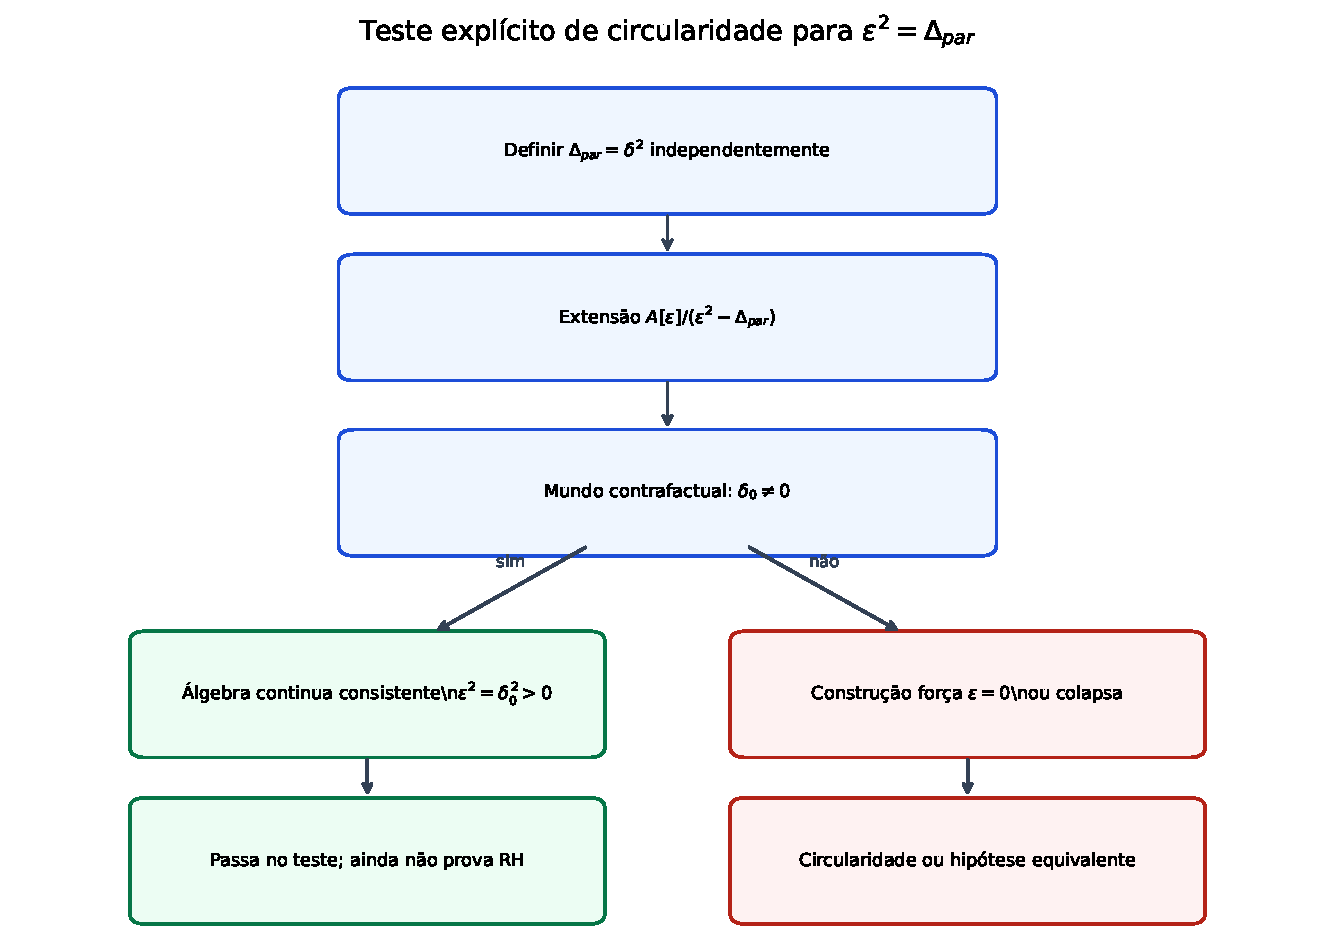
\includegraphics[width=.94\linewidth]{11-teste-circularidade.pdf}\caption{Teste contrafactual obrigatório.}\end{figure}

\section{Classificação final}
\begin{figure}[ht]\centering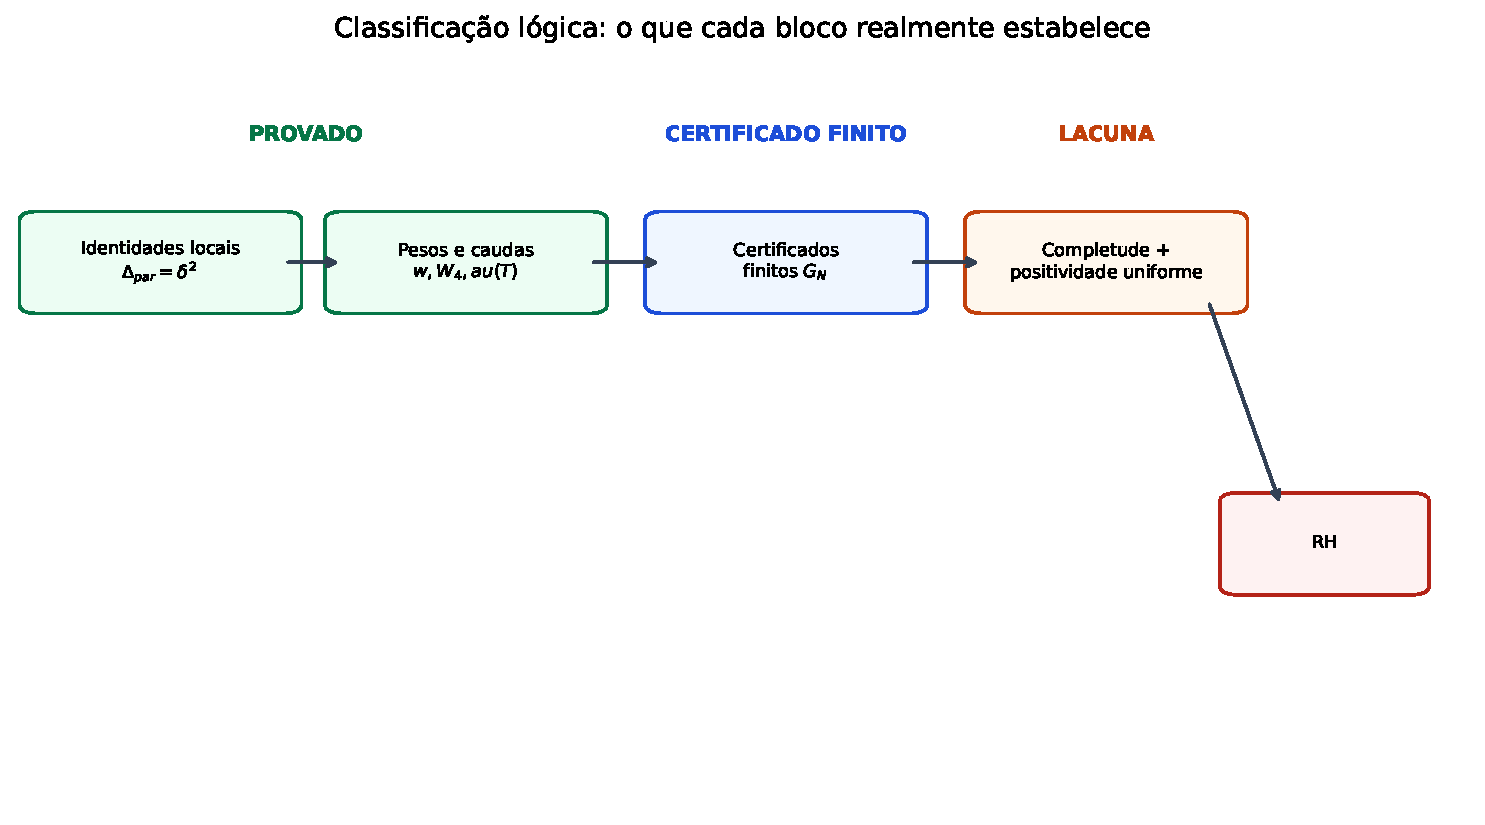
\includegraphics[width=.98\linewidth]{09-status-logico.pdf}\caption{Separação dos níveis de evidência.}\end{figure}
\begin{longtable}{p{.19\linewidth}p{.72\linewidth}}
\toprule Status & Conteúdo \\\midrule
Provado & Identidades de $R_c,R_\pm$, $\Dpar=\delta^2$, positividade local de $w$, simetrias e expansões assintóticas elementares.\\
Certificado finito & Qualquer verificação computacional em altura ou dimensão explicitamente limitada, desde que acompanhada de aritmética intervalar e dados reproduzíveis.\\
Equivalente & $\Drad=0$, positividade de Weil para todas as funções admissíveis e positividade de toda uma família completa de Gram com passagem ao limite.\\
Conjectural & Núcleo primo não derivado, métrica destrutiva, conservação que exclua $\epsilon\ne0$ e extensões para outros problemas do milênio.\\
\bottomrule
\end{longtable}

\section{Conclusão}
O detector local e sua análise multiescala são matematicamente úteis e auditáveis. O ponto de ruptura permanece a obtenção, por meios independentes da RH, de uma lei coerciva que anule o defeito global. O programa de pesquisa é válido como estrutura falsificável; não constitui solução da RH sem essa ponte.

\end{document}
